\documentclass[english, 11pt]{article}
\usepackage[T1]{fontenc}
\usepackage[latin9]{inputenc}
\usepackage[top = 2cm, left = 2.5cm, right = 2.5cm, bottom = 2cm]{geometry}
\usepackage{enumitem}
\usepackage{amsmath}
\usepackage{amsfonts}
\usepackage{amstext}
\usepackage{mdframed}
\usepackage{graphicx}
\usepackage{subcaption} %Added this library


\usepackage{bbm}
\makeatletter
\@ifundefined{date}{}{\date{}}
\usepackage{tikz}
\usetikzlibrary{quotes, angles, decorations.markings, intersections}
\usetikzlibrary{calc,patterns,angles,quotes, 3d, intersections, positioning, shapes, automata, positioning}
\usepackage{wasysym}
\makeatother
\usepackage{babel}
\usepackage{color}
\usepackage{graphicx}
\usepackage{hyperref}

\hypersetup{
	colorlinks,
	citecolor=black,
	filecolor=black,
	linkcolor=black,
	urlcolor=black
}


\newcommand{\tbox}[1]{\noindent\fbox{\parbox{\textwidth}{#1}}}

\setlength{\parindent}{0pt}

\begin{document}
\noindent\tbox{
\textbf{CS 208 : Automata Theory and Logic} \hfill DATE
\begin{center}
  \huge Lecture - 22 \\ % change lecture number
  \Large Topic: Minimal DFAs % Short topic description
\end{center}
\textit{Scribed by}: Saksham Rathi % <NAME> (<Roll Number>)

\textit{Checked and compiled by}: Kartik P. Gokhale % <TA Name>
}

\paragraph{Disclaimer.} {\bfseries Please note this document has not received
the usual scrutiny that formal publications enjoy. This may be
distributed outside this class only with the permission of the
instructor.}


\section{Minimum States in a DFA}
So, far we have dealt with DFA, NFA without $\epsilon$, NFA with $\epsilon$ and Regular Expressions. We have also seen that all of them are equivalent and inter-convertible and represent regular languages.


Consider the language which consists of all strings which are terminated by one. The regular expression for this will be: $(0+1)^{*}1$. Here is a 2-state DFA for the same language:

\begin{figure}[htbp]
\begin{center}
    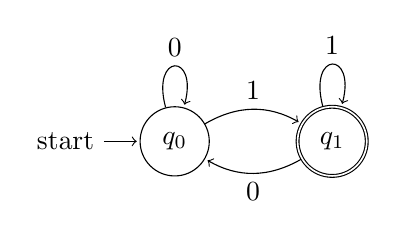
\begin{tikzpicture}[shorten >=1pt,node distance=2cm,on grid,auto]
    
      \node[state,initial]  (q_0)                      {$q_0$};
      \node[state,accepting]          (q_1) [right=of q_0] {$q_1$};
    
      \path[->] (q_0) edge  [bend left]            node        {1} (q_1)
                      edge [loop above] node        {0} ()
                (q_1) edge [bend left]           node        {0} (q_0)
                      edge [loop above] node        {1} ();
    \end{tikzpicture}
\end{center}
\caption{2-state DFA for the language}
\label{fig:figfromtikz}
\end{figure}

The above DFA has two states $q_0$ and $q_1$. $q_0$ is reached when the last seen letter was 0 (also at the start). $q_1$ is reached when the last seen letter was 1 (also, it is an accepting state).


We can even construct a 4-state DFA for the same language. Here is an example:

\begin{figure}[htbp]
\begin{center}
    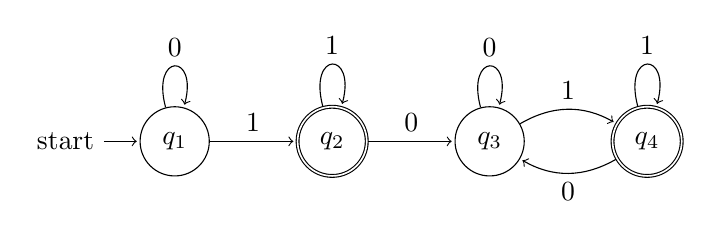
\begin{tikzpicture}[shorten >=1pt,node distance=2cm,on grid,auto]
    
      \node[state,initial]  (q_1)                      {$q_1$};
      \node[state,accepting]          (q_2) [right=of q_1] {$q_2$};
      \node[state]          (q_3) [right=of q_2] {$q_3$};
      \node[state,accepting]          (q_4) [right=of q_3] {$q_4$};
    
      \path[->] (q_1) edge            node        {1} (q_2)
                      edge [loop above] node        {0} ()
                (q_2) edge          node        {0} (q_3)
                      edge [loop above] node        {1} ()
                      (q_3) edge  [bend left]        node        {1} (q_4)
                      edge [loop above] node        {0} ()
                      (q_4) edge [bend left]         node        {0} (q_3)
                      edge [loop above] node        {1} ();
    \end{tikzpicture}
\end{center}
\caption{4-state DFA for the language}
\label{fig:4state}
\end{figure}


The above DFA has four states $q_1$, $q_2$, $q_3$, $q_4$.
\begin{itemize}
    \item $q_1$: Last letter 0 and no 1s so far
    \item $q_2$: Last letter 1 and no 101 seen so far
    \item $q_3$: Last letter 0 and more than one 1s seen so far
    \item $q_4$: Last letter 1
\end{itemize}


One can construct many more 4-state DFAs for the same language. Above is another example.



\begin{figure}[htbp]
\begin{center}
    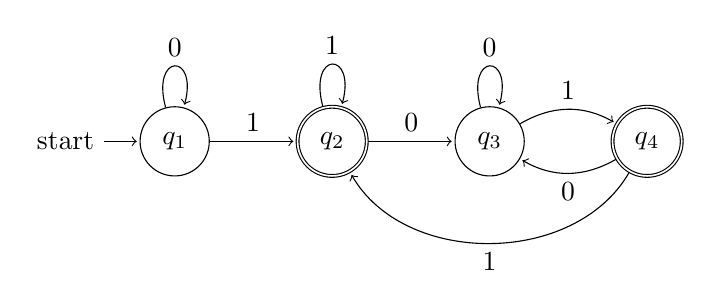
\begin{tikzpicture}[shorten >=1pt,node distance=2cm,on grid,auto]
    
      \node[state,initial]  (q_1)                      {$q_1$};
      \node[state,accepting]          (q_2) [right=of q_1] {$q_2$};
      \node[state]          (q_3) [right=of q_2] {$q_3$};
      \node[state,accepting]          (q_4) [right=of q_3] {$q_4$};
    
      \path[->] (q_1) edge            node        {1} (q_2)
                      edge [loop above] node        {0} ()
                (q_2) edge          node        {0} (q_3)
                      edge [loop above] node        {1} ()
                      (q_3) edge  [bend left]        node        {1} (q_4)
                      edge [loop above] node        {0} ()
                      (q_4) edge [bend left]         node        {0} (q_3)
                      edge [bend left=60]  node        {1} (q_2);
    \end{tikzpicture}
\end{center}
\caption{Another 4-state DFA for the same language}
\label{fig:4state1}
\end{figure}



A natural question which comes to our mind is that can we construct another 2-state DFA for this language. One can find through trial and error, that this is not possible.


Is one state DFA possible for this language? Let us assume that this is possible. Two cases arise. If that state is accepting, then it will also accept $\epsilon$, which is not possible. If that state is not accepting, then the language will be empty. We have arrived at a contradiction. Hence, one state DFA is not possible for this language.


Therefore, for this language, the minimum states in any DFA can be 2. We also observe that number of such 2-state DFAs is 1. So, we will now claim that for every language, the number of minimal DFAs is 1 and try to prove this. Before we prove this, we will introduce the notion of indistinguishability.


\section{Indistinguishability}
Two states of a DFA $q_i$ and $q_j$ are considered indistinguishable, if $\forall w \in \Sigma^*$, we start with $q_i$, process $w$ and reach $q_i'$ and we start with $q_j$, process $w$ and reach $q_j'$, then either $q_i' \in F \text{ and } q_j' \in F$ or $q_i' \notin F \text{ and } q_j' \notin F$, where $F$ is the set of all final states of the DFA. So, we are basically changing the start states and checking whether we reach the same type of states or not through the same string.


This relation is denoted by $\equiv$. It has the following properties:
\begin{itemize}
    \item It is \textbf{reflexive}. It is clear to see that every state is indistinguishable to itself, as it will reach a particular state on seeing $w$. (Due to the nature of a DFA)
    \item Also, it is clear to see that this relation is \textbf{symmetric}.
    \item This relation is also \textbf{transitive}. We can prove this by contradiction. Let us assume that $(q_i \equiv q_j) \wedge (q_j \equiv q_k)$ but $q_i \not\equiv q_k$. Then $\exists w$ such that $q_i' \in F$ and $q_k' \notin F$, where $q_i'$ and $q_k'$ are the states we reach from $q_i$ and $q_k$ respectively on seeing $w$. From the equivalence of $q_i$ and $q_j$, we have $q_j' \in F$ but from the equivalence of $q_j$ and $q_k$, we have $q_j' \notin F$, where $q_j'$ is the state that we reach from $q_j$ on seeing $w$. Hence, we have arrived at a contradiction. Therefore, this relation is transitive. 
    \item A relation which is reflexive, symmetric and transitive, is \textbf{equivalent}. Thus the states of the DFA, on which this relation is defined can be partitioned into equivalence classes. 
\end{itemize}


In the above example (Figure: \ref{fig:4state}), $q_1$ and $q_3$ belong to the same equivalence class, and $q_2$ and $q_4$ also belong to another equivalence class. Let us now try to construct a 2-state DFA from the above 4-state DFA example (Figure: \ref{fig:4state}). We will choose, one element each from both of the equivalence classes. Let us take $q_1$ from the first class and $q_4$ from the second class. 

\begin{figure}[htbp]
\begin{center}
    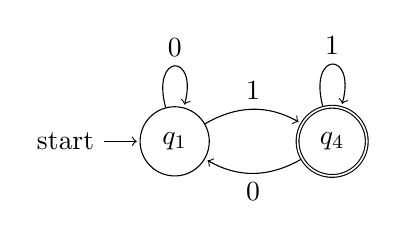
\begin{tikzpicture}[shorten >=1pt,node distance=2cm,on grid,auto]
    
      \node[state,initial]  (q_1)                      {$q_1$};
      \node[state,accepting]          (q_4) [right=of q_1] {$q_4$};
    
      \path[->] (q_1) edge  [bend left]            node        {1} (q_4)
                      edge [loop above] node        {0} ()
                (q_4) edge [bend left]           node        {0} (q_1)
                      edge [loop above] node        {1} ();
    \end{tikzpicture}
\end{center}
\caption{2-state DFA constructed from the 4-state DFA}
\label{fig:2sta}
\end{figure}

From $q_1$, if we see a 0, we land at $q_1$ itself. If we see a 1, we would have landed at $q_2$, but since $q_2$ and $q_4$ are equivalent, we replace $q_2$ by $q_4$. Similarly, from $q_4$, if we see a 1, we remain at $q_4$, but if we see a 0, we would have landed at $q_3$, but since $q_1$ and $q_3$ are equivalent, we replace $q_3$ by $q_1$. Also, $q_2$ and $q_4$ both were acceptable earlier, now $q_4$ is acceptable. 


So, through these equivalence classes, we have minimized our 4-state DFA into a 2-state DFA, and also this 2-state DFA is structurally the same as the previous one (Figure: \ref{fig:figfromtikz}), thus again making us think that the claim that there is a single minimal DFA for every language might be correct. 


Another interesting thing we observe is that an accepting state cannot be indistinguishable from a non-accepting state. We can take $w = \epsilon$, and observe that the states we reach from this pair of states do not satisfy the definition of indistinguishability relation. However, an initial state and a non-initial state can belong to the same equivalence class. (For example, above $q_1$ and $q_3$ belonged to the same class.)


Now, several important questions arise. How can we find the equivalence classes of this relation? When we will come to know that we cannot compress our DFA further (by compress, we mean reducing the number of states of the DFA)? How can we prove our claim that the minimal DFA will be unique?


We will try to answer all these questions subsequently. Let us start with the easiest one.


\section{Equivalence classes of Indistinguishability relation}
Now, we will develop an algorithm to find the equivalence classes of this relation.


Firstly, we should keep in mind our previous observation that an accepting state cannot be indistinguishable from a non-accepting state. That is $q_i \not\equiv q_j \text{ }\forall q_i \in F \text{ and } q_j \in (Q\textbackslash F)$, where $Q$ is the set of all states of the DFA. 


Suppose, we find two states $q_s$ and $q_t$ which are distinguishable. Thus there exists a string w such that $q_s$ leads to an accepting state but $q_t$ leads to a non-accepting state. 

\begin{figure}[htbp]
\begin{center}
    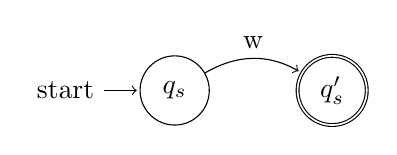
\begin{tikzpicture}[shorten >=1pt,node distance=2cm,on grid,auto]
    
      \node[state,initial]  (q_s)                      {$q_s$};
      \node[state,accepting]          (q_s') [right=of q_s] {$q_s'$};
    
      \path[->] (q_s) edge  [bend left]            node        {w} (q_s');
    \end{tikzpicture}
\end{center}
\label{fig:2sta}
\end{figure}


\begin{figure}[htbp]
\begin{center}
    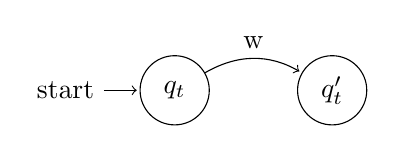
\begin{tikzpicture}[shorten >=1pt,node distance=2cm,on grid,auto]
    
      \node[state,initial]  (q_t)                      {$q_t$};
      \node[state]          (q_t') [right=of q_t] {$q_t'$};
    
      \path[->] (q_t) edge  [bend left]            node        {w} (q_t');
    \end{tikzpicture}
\end{center}
\label{fig:2sta}
\end{figure}


Now, $w$ can be decomposed into $a_1a_2\dots a_n$, where $|w| = n$.

\clearpage
\begin{figure}[htbp]
\begin{center}
    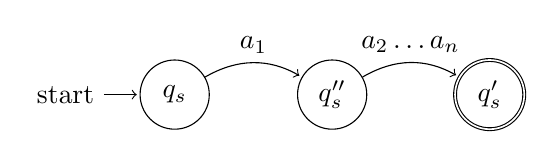
\begin{tikzpicture}[shorten >=1pt,node distance=2cm,on grid,auto]
    
      \node[state,initial]  (q_s)                      {$q_s$};
      \node[state]  (q_s'')       [right=of q_s]               {$q_s''$};
      \node[state,accepting]          (q_s') [right=of q_s''] {$q_s'$};
    
      \path[->] (q_s) edge  [bend left]            node        {$a_1$} (q_s'')
                (q_s'') edge  [bend left]            node        {$a_2\dots a_n$} (q_s');
    \end{tikzpicture}
\end{center}
\label{fig:2sta}
\end{figure}
\begin{figure}[htbp]
\begin{center}
    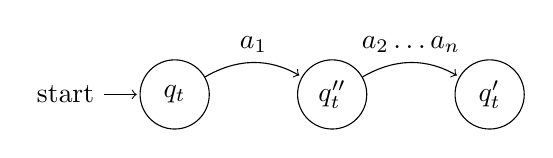
\begin{tikzpicture}[shorten >=1pt,node distance=2cm,on grid,auto]
    
      \node[state,initial]  (q_t)                      {$q_t$};
      \node[state]  (q_t'')       [right=of q_t]               {$q_t''$};
      \node[state]          (q_t') [right=of q_t''] {$q_t'$};
    
      \path[->] (q_t) edge  [bend left]            node        {$a_1$} (q_t'')
                (q_t'') edge  [bend left]            node        {$a_2\dots a_n$} (q_t');
    \end{tikzpicture}
\end{center}
\label{fig:2sta}
\end{figure}

From, the above figures, one can observe that $q_s''$ and $q_t''$ are also distinguishable, where $w' = a_2\dots a_n$ is the string which is making them distinguishable.


Thus, we can observe that for all states $q_i$ and $q_j$ such that $q_i \not\equiv q_j$ and for all $a \in \Sigma$, such that $q_s$ on seeing $a$ lands at $q_i$ and $q_t$ on seeing $a$ lands at $q_j$ then $q_s$ will be distinguishable with $q_t$, where $q_s$ and $q_t$ are two states of the DFA.(We are basically extending $w' = a + w$.)


Therefore using a distinguishable pair, we have found another one. This is the basis of our algorithm. We initialize our set with all the pairs, where one state belongs to the set of accepting states and other state does not belong to the set of non accepting states. And then through the above step, we keep on increasing the size of this set. (Note that this algorithm is not exponential, because there are only $\binom{n}{2}$ pairs possible, and we do need to check an already visited pair.)


\begin{center}
    \begin{tikzpicture}
        % Add text above and left of the box
        \node at (-0.5,6.5) {$q_1$};
        \node at (-0.5,5.5) {$q_2$};
        \node at (-0.5,2.5) {$.$};
        \node at (-0.5,2.0) {$.$};
        \node at (-0.5,1.5) {$.$};
        \node at (-0.5,0.5) {$q_n$};

        \node at (0.5, 7.5) {$q_1$};
        \node at (1.5, 7.5) {$q_2$};
        \node at (3.5, 7.5) {$.$};
        \node at (4, 7.5) {$.$};
        \node at (4.5, 7.5) {$.$};
        \node at (6.5, 7.5) {$q_n$};
        
        % Draw the box
        \draw (0,0) rectangle (7,7);
        
        % Draw the diagonal
        \draw (0,7) -- (7,0);
        
        % Add text inside the box
        \node at (1.5,1.5) {X};
        \node at (3,1.5) {X};
        \node at (3,3.5) {X};
        \node at (0.5,3.5) {X};
    \end{tikzpicture}
\end{center}



We stop the process, when no more crosses can be inserted.


Now, it is quite natural for us to ask the question that whether our algorithm is correct or not i.e. can we still find a pair of distinguishable states, which are not detected even after our algorithm finishes?


\textbf{Proof: }Let us assume that there are two states $q_s$ and $q_t$ which are distinguishable but not recognized by our algorithm. By definition, there exists a string $w$ such that $q_s$ leads to an accepting state on seeing $w$ and $q_t$ reaches a non-accepting state.


\begin{figure}[htbp]
    \begin{subfigure}{0.45\textwidth}
        \begin{center}
            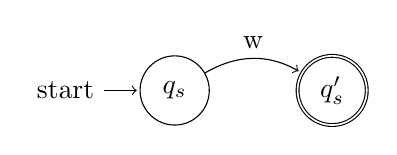
\begin{tikzpicture}[shorten >=1pt,node distance=2cm,on grid,auto]
                \node[state,initial]  (q_s) {$q_s$};
                \node[state,accepting] (q_s') [right=of q_s] {$q_s'$};
                \path[->] (q_s) edge [bend left] node {w} (q_s');
            \end{tikzpicture}
            \label{fig:2sta1}
        \end{center}
    \end{subfigure}
    \hspace{1cm} % Adjust the space between the two figures
    \begin{subfigure}{0.45\textwidth}
        \begin{center}
            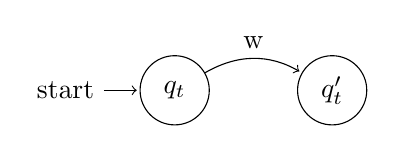
\begin{tikzpicture}[shorten >=1pt,node distance=2cm,on grid,auto]
                \node[state,initial] (q_t) {$q_t$};
                \node[state] (q_t') [right=of q_t] {$q_t'$};
                \path[->] (q_t) edge [bend left] node {w} (q_t');
            \end{tikzpicture}
            \label{fig:2sta2}
        \end{center}
    \end{subfigure}
    \label{fig:2sta}
\end{figure}


Now $w$ can be written as $a_1a_2\dots a_n$, where $|w| = n$. And also assume that we reach $q_s''$ and $q_t''$ on seeing $a_1$ from $q_s$ and $q_t$ respectively. It is clear that, if our algorithm has not detected $q_s$ and $q_t$ as distinguishable, then it would not even have detected $q_s''$ and $q_t''$ as a distinguishable pair. (Because, if it would have done, then the next step would have been to make $q_s$ and $q_t$ as distinguishable.)



\begin{figure}[htbp]
    \begin{subfigure}{0.45\textwidth}
        \begin{center}
            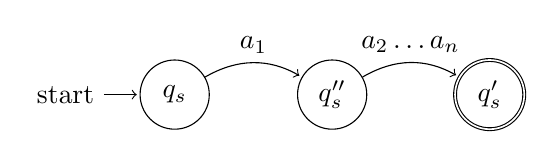
\begin{tikzpicture}[shorten >=1pt,node distance=2cm,on grid,auto]
    
      \node[state,initial]  (q_s)                      {$q_s$};
      \node[state]  (q_s'')       [right=of q_s]               {$q_s''$};
      \node[state,accepting]          (q_s') [right=of q_s''] {$q_s'$};
    
      \path[->] (q_s) edge  [bend left]            node        {$a_1$} (q_s'')
                (q_s'') edge  [bend left]            node        {$a_2\dots a_n$} (q_s');
    \end{tikzpicture}
            \label{fig:2sta1}
        \end{center}
    \end{subfigure}
    \hspace{1cm} % Adjust the space between the two figures
    \begin{subfigure}{0.45\textwidth}
        \begin{center}
            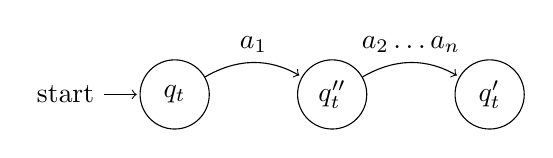
\begin{tikzpicture}[shorten >=1pt,node distance=2cm,on grid,auto]
    
      \node[state,initial]  (q_t)                      {$q_t$};
      \node[state]  (q_t'')       [right=of q_t]               {$q_t''$};
      \node[state]          (q_t') [right=of q_t''] {$q_t'$};
    
      \path[->] (q_t) edge  [bend left]            node        {$a_1$} (q_t'')
                (q_t'') edge  [bend left]            node        {$a_2\dots a_n$} (q_t');
    \end{tikzpicture}
            \label{fig:2sta2}
        \end{center}
    \end{subfigure}
    \label{fig:2sta}
\end{figure}


Now, we will inductively move forward  our algorithm. Thus $q_s'''$ and $q_t'''$ would not also be detected as distinguishable after our algorithm finishes. But clearly, this is not possible, because our algorithm initializes the set of pairs of \{accepting, non-accepting\} states and then it's first step is to move backwards. So, it would have marked $q_s'''$ and $q_t'''$ as distinguishable in the first step itself.


\begin{figure}[htbp]
    \begin{subfigure}{0.45\textwidth}
        \begin{center}
            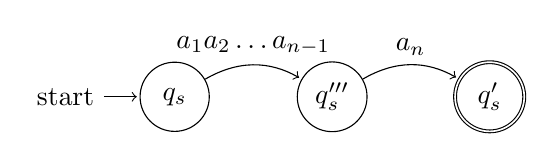
\begin{tikzpicture}[shorten >=1pt,node distance=2cm,on grid,auto]
    
      \node[state,initial]  (q_s)                      {$q_s$};
      \node[state]  (q_s'')       [right=of q_s]               {$q_s'''$};
      \node[state,accepting]          (q_s') [right=of q_s''] {$q_s'$};
    
      \path[->] (q_s) edge  [bend left]            node        {$a_1a_2\dots a_{n-1}$} (q_s'')
                (q_s'') edge  [bend left]            node        {$a_n$} (q_s');
    \end{tikzpicture}
            \label{fig:2sta1}
        \end{center}
    \end{subfigure}
    \hspace{1cm} % Adjust the space between the two figures
    \begin{subfigure}{0.45\textwidth}
        \begin{center}
            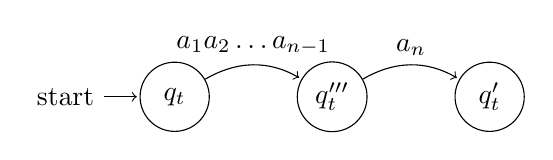
\begin{tikzpicture}[shorten >=1pt,node distance=2cm,on grid,auto]
    
      \node[state,initial]  (q_t)                      {$q_t$};
      \node[state]  (q_t'')       [right=of q_t]               {$q_t'''$};
      \node[state]          (q_t') [right=of q_t''] {$q_t'$};
    
      \path[->] (q_t) edge  [bend left]            node        {$a_1a_2\dots a_{n-1}$} (q_t'')
                (q_t'') edge  [bend left]            node        {$a_n$} (q_t');
    \end{tikzpicture}
            \label{fig:2sta2}
        \end{center}
    \end{subfigure}
    \label{fig:2sta}
\end{figure}


We have achieved contradiction. Therefore, we can safely conclude that our algorithm terminates and is also correct.


Now, once our algorithm detects all pairs of distinguishable states, we can choose equivalence classes of the indistinguishability relation. (Then, we can choose one representative from each class and move forward with our proof of existence of a unique minimal DFA.)


It is worth noting that distinguishability is not an equivalent relation. It is not even reflexive. It is also not transitive. But, it is indeed symmetric. And also, it proved out to be very useful for finding these equivalence classes. 


Now, we will move forward with the remaining two questions, that can we compress a given DFA further and does there exist any other minimal DFA?


% \definecolor{ududff}{rgb}{0.30196078431372547,0.30196078431372547,1}
% \definecolor{xdxdff}{rgb}{0.49019607843137253,0.49019607843137253,1}
% \begin{tikzpicture}[line cap=round,line join=round,>=triangle 45,x=1cm,y=1cm]
% \begin{axis}[
% x=1cm,y=1cm,
% axis lines=middle,
% ymajorgrids=true,
% xmajorgrids=true,
% xmin=-13.4,
% xmax=13.4,
% ymin=-11.07,
% ymax=6.65,
% xtick={-13,-12,...,13},
% ytick={-11,-10,...,6},]
% \clip(-13.4,-11.07) rectangle (13.4,6.65);
% \draw [line width=2pt] (2,-11.07) -- (2,6.65);
% \begin{scriptsize}
% \draw [fill=xdxdff] (2,0) circle (2.5pt);
% \draw[color=xdxdff] (2.16,0.42) node {$A$};
% \draw [fill=ududff] (2,5) circle (2.5pt);
% \draw[color=ududff] (2.16,5.42) node {$B$};
% \draw[color=black] (1.76,6.4) node {$f$};
% \end{scriptsize}
% \end{axis}
% \end{tikzpicture}

% The two-state DFA will be as shown below:
% \begin{figure}[h!]
% %     % code for subfigure, label them for using references
%      \centering
%     \includegraphics[width=\textwidth]{Screenshot 2024-03-11 at 7.16.54 PM.png}
%      \caption{2-state DFA}
%      \label{fig:image}
% \end{figure}


% \section{Section title}
%  Here is where you insert your proper notes.
% \subsection{Subsection title}

% Figures can be drawn using TikZ (see link below) or can be included as
% a PDF file.

% Here's how to include a figure (\ref{fig:figfrompdf}) from a PDF file
% \begin{figure}[htbp]
%   \begin{center}
%   \includegraphics[width=.7\textwidth]{L1slides_p3.pdf}
%   \end{center}
%   \caption{A simple figure}
%   \label{fig:figfrompdf}
% \end{figure}

% Here's a figure of an automaton (Fig.~\ref{fig:figfromtikz}) drawn using
% \LaTeX{}. You do not have to use TikZ, but if you are free and bored,
% please try it out for vector graphics with amazing user-controlled
% precision.
% \begin{figure}[htbp]
% \begin{center}
%     \begin{tikzpicture}[shorten >=1pt,node distance=2cm,on grid,auto]
    
%       \node[state,initial]  (q_0)                      {$q_0$};
%       \node[state]          (q_1) [above right=of q_0] {$q_1$};
%       \node[state]          (q_2) [below right=of q_0] {$q_2$};
%       \node[state,accepting](q_3) [below right=of q_1] {$q_3$};
    
%       \path[->] (q_0) edge              node        {0} (q_1)
%                       edge              node [swap] {1} (q_2)
%                 (q_1) edge              node        {1} (q_3)
%                       edge [loop above] node        {0} ()
%                 (q_2) edge              node [swap] {0} (q_3)
%                       edge [loop below] node        {1} ();
%     \end{tikzpicture}
% \end{center}
% \caption{An automaton}
% \label{fig:figfromtikz}
% \end{figure}

% TIKZ reference manual:  \href{https://tikz.dev/}{Click here}

% Automata in \LaTeX{}: \href{https://tikz.dev/library-automata}{Click here}

\end{document}